\documentclass[11pt]{article}

\usepackage{amsmath}
\usepackage{amssymb}
\usepackage{color}
\usepackage{cancel}
\usepackage{listings}
\usepackage{xcolor}
\usepackage{graphicx}

\definecolor{codegreen}{rgb}{0,0.6,0}
\definecolor{codegray}{rgb}{0.5,0.5,0.5}
\definecolor{codepurple}{rgb}{0.58,0,0.82}
\definecolor{backcolour}{rgb}{0.95,0.95,0.92}

\lstdefinestyle{mystyle}
{
    backgroundcolor=\color{backcolour},   
    commentstyle=\color{codegreen},
    keywordstyle=\color{magenta},
    numberstyle=\tiny\color{codegray},
    stringstyle=\color{codepurple},
    basicstyle=\ttfamily\footnotesize,
    breakatwhitespace=false,         
    breaklines=true,                 
    captionpos=b,                    
    keepspaces=true,                 
    numbers=left,                    
    numbersep=5pt,                  
    showspaces=false,                
    showstringspaces=false,
    showtabs=false,                  
    tabsize=2
}

\lstset{style=mystyle}

\textwidth=6.5in
\textheight=9.3in
\topmargin=-0.8in
\headheight=15.75pt
\headsep=.35in
\oddsidemargin=0.0in
\evensidemargin=0.0in

\newcommand{\Complex}{\mathbb{C}}
\newcommand{\Real}{\mathbb{R}}
\newcommand{\Dpt}{D_{+t}}
\newcommand{\Dmt}{D_{-t}}
\newcommand{\Dzt}{D_{0t}}
\newcommand{\Dpx}{D_{+x}}
\newcommand{\dpx}{\Delta_{+x}}
\newcommand{\Dmx}{D_{-x}}
\newcommand{\dmx}{\Delta_{-x}}
\newcommand{\Dzx}{D_{0x}}
\newcommand{\Oc}{\mathcal{O}}
\newcommand{\dx}{\Delta x}
\newcommand{\dt}{\Delta t}
\newcommand{\bra}[1]{\left(#1\right)}
\newcommand{\inte}[1]{\int_0^1 #1\, dx}
\newcommand{\vj}{v_j}
\newcommand{\vnj}{v^n_j}
\newcommand{\vnpjm}{v^{n+1}_{j-1}}
\newcommand{\vnpjp}{v^{n+1}_{j+1}}
\newcommand{\vnpj}{v^{n+1}_{j}}
\newcommand{\vnjm}{v^{n}_{j-1}}
\newcommand{\vnjp}{v^{n}_{j+1}}
\newcommand{\njmh}{\nu_{j-\frac{1}{2}}}
\newcommand{\njph}{\nu_{j+\frac{1}{2}}}
\newcommand{\dint}[1]{\sum_{j=0}^{N-1}#1}
\newcommand{\h}{\frac{1}{2}}

\begin{document}
\begin{flushright}
\small{MATH-6840\\
Vignesh Ramakrishnan\\
{\bf Due: Monday March 28, 2022}}
\end{flushright}

\begin{center}
\large{Problem Set 7}\\
\end{center}

\begin{enumerate}
  %%%%%
  %%%%%
  %%%%%
  \item (25 pts.) {\color{red}Consider the variable coefficient diffusion equation} 
  \[
    u_t=(Du_x)_x, \qquad 0 < x < 1, \qquad t >0
  \]
  {\color{red}where $D>0$ is a function of $x$, with initial conditions $u(x,0)=u_0(x)$ and subject to boundary conditions $u_x(0,t) = 0$, $u(1,t) = 0$.}

  %%%
  \begin{enumerate}
    \item {\color{blue}Show that this problem is well-posed by proving the energy estimate}
    \[
      \frac{d}{dt}||u||^2 \le 0,
    \]
    {\color{blue}where} $||u||^2=(u,u)=\int_0^1 u^2\, dx$.
    \begin{align*}
        u_t =& \ \bra{Du_x}_x \\
        u\,u_t =& \ u\,\bra{Du_x}_x \\
        \inte{u\,u_t} =& \inte{u\,\bra{Du_x}_x} \\
        \inte{\frac{1}{2}\frac{d||u||^2}{dt}} =& \ \cancel{u(1)}\bra{Du_x(1)} - u(0)\bra{D\cancel{u_x(0)}} - \inte{u_xDu_x}\\
        \inte{\frac{1}{2}\frac{d||u||^2}{dt}} =& \ -\inte{D\bra{u_x}^2} 
    \end{align*}
    Here, $D\geq0$ and $\bra{u_x}^2 \geq 0$ always and hence,
    \[
    \frac{1}{2}\frac{d||u||^2}{dt} \leq 0
    \]
    Thus, this PDE is well posed.
    %
    \item {\color{blue}Propose a computational grid, a semi-discretization of the PDE in space, and a treatment of the boundary conditions for which you can prove a discrete energy estimate of the form $\frac{d}{dt}||u||^2_h \le 0$ for an appropriately defined discrete norm $||\cdot ||_h$. Prove your discrete energy estimate.}
    \begin{align*}
        \dx =& \ 1/N \\
        x_j =& \ (j-\h)\dx, \; j=0,1,2,\ldots \ldots ,N 
    \end{align*}
    and here, $\Dmx v_j = \frac{v_{j+\h}-v_{j-\h}}{\dx}$
    \begin{align*}
        \frac{d\vj}{dt} =& \ \Dpx\bra{\nu_{j-\frac{1}{2}}\Dmx\vj} \\
        \vj\,\frac{d\vj}{dt} =& \ \vj \Dpx\bra{\nu_{j-\frac{1}{2}}\Dmx\vj} \\
        \dx\dint{\frac{1}{2}\frac{d||\vj||^2_h}{dt}} =& \ \dx\dint{\vj\Dpx\bra{\nu_{j-\frac{1}{2}}\Dmx\vj}} \\
        \dx\dint{\frac{1}{2}\frac{d||\vj||^2_h}{dt}} =& \ \frac{\dx}{\dx^2}\dint{\vj\dpx\bra{\nu_{j-\frac{1}{2}}\dmx\vj}}
    \end{align*}
    Using summation by parts, we can simplify and get to the form
    \begin{align*}
       \dx\dint{\frac{1}{2}\frac{d||\vj||^2_h}{dt}} =& \ \frac{\dx}{\dx^2}\bra{\cancel{v_N}\bra{\nu_{N-\frac{1}{2}}\dmx v_N} -v_0\nu_{-\frac{1}{2}}\dmx v_0 - \dint{\bra{\njph \dmx v_{j+1}}\dpx\vj}} \\
       \dint{\frac{1}{2}\frac{d||\vj||^2_h}{dt}} =& \bra{-\frac{1}{\dx}v_0\nu_{-\frac{1}{2}}\cancel{\Dmx v_0} - \frac{1}{\dx^2}\dint{\bra{\njph\bra{\dpx\vj}^2}}} \\
    \end{align*}
    Since $\njph\geq0$ and $\bra{\dpx\vj}^2\geq0$, 
    \[
    \frac{d||\vj||^2_h}{dt} \leq 0
    \]
    %
    \item {\color{blue}Prove a fully discrete energy estimate for Crank-Nicolson integration of the scheme from part (b) above.}
    \begin{align*}
    \frac{v^{n+1}_j - v^n_j}{\dt} =& \ \Dpx\bra{\nu_{j-\h}\Dmx}\frac{v^{n+1}_j+v^n_j}{2}\\
    \bra{v^{n+1}_j}^2 - \bra{v^n_j}^2 =& \ \dt \Dpx\bra{\nu_{j-\h}\Dmx}\frac{v^{n+1}_j+v^n_j}{2} \bra{v^{n+1}_j+v^n_j} \\
    \bra{v^{n+1}_j}^2 - \bra{v^n_j}^2 =& \ \frac{\dt}{4}\Dpx\bra{\nu_{j-\h}\Dmx}v^{n+\h}_j v^{n+\h}_j \\
    \dx \dint{\bra{v^{n+1}_j}^2 - \bra{v^n_j}^2} =& \ -\dx\dint{\bra{\Dpx v^{n+\h}_j, \Dpx\bra{\nu_{j-\h}v^{n+\h}_j}}}++ \left[v^{n+\h}_j\Dpx v^{n+\h}_j\right]_{j=0}^{j=N}\\
    \end{align*}
    %
    \item {\color{blue}Write a code to implement the scheme in part (d). Demonstrate second-order convergence using a manufactured solution.} \\
    Method of manufactured solutions is used to verify second-order of convergence.
    \begin{align*}
        u_{ex} =& \ \cos{\bra{\frac{\pi x}{2}}}\sin{t}, \, u_{ex}(x=1,t)=0 \\
        u_t =& \ \cos{\bra{\frac{\pi x}{2}}}\cos{t} \\
        u_x =& \ -\frac{\pi}{2}\sin{\bra{\frac{\pi x}{2}}}\sin{t}, \, u_x(x=0,t) = 0 \\
        u_{xx} =& \ -\frac{\pi^2}{4}\cos{\bra{\frac{\pi x}{2}}}\sin{t}
    \end{align*}
    \begin{align*}
        u_t -\bra{\nu u_x}_x =& \ u_t - \bra{\nu_x u_x + \nu u_{xx}} = f(x,t) 
    \end{align*}
    This solution satisfies the boundary conditions specified in the problem. The discrete set of equations for the Crank-Nicholson scheme is, 
    \begin{align*}
        \Dpt \vnj =& \ \Dpx\bra{\njmh\Dmx}\bra{\frac{\vnpj + \vnj}{2}} + \bra{\frac{f^{n+1}_j+f^n_j}{2}} \\
        \Dpt \vnj =& \ \frac{1}{2}\Dpx\bra{\njmh\vnpj} + \frac{1}{2}\Dpx\bra{\njmh\vnj} + \bra{\frac{f^{n+1}_j+f^n_j}{2}}
    \end{align*}
    Setting $\hat{F} = \bra{\frac{f^{n+1}_j+f^n_j}{2}}$ and $\Gamma = \frac{\dt}{\dx^2}$, this simplifies to,
    \begin{align*}
        -\frac{\Gamma}{2}\njmh\vnpjm +& \bra{1+\frac{\Gamma}{2}\bra{\njph+\njmh}}\vnpj -\frac{\Gamma}{2}\njph\vnpjp = \\
        & \frac{\Gamma}{2}\njmh\vnjm + \bra{1-\frac{\Gamma}{2}\bra{\njph+\njmh}}\vnj + \frac{\Gamma}{2}\njph \vnjp + \dt \hat{F} \\
        & j=1,2,\ldots \ldots, N-1
    \end{align*}
    Boundary conditions are given by,
    \begin{align*}
        \frac{v^{n+1}_{1} - v^{n+1}_{0}}{\dx} =& \ 0, \; & \frac{v^{n+1}_{N}+v^{n+1}_{N-1}}{2} =& 0 
    \end{align*}
    The code is shown in Listing~\ref{lst:CN_HE}. The order of convergence is shown in Fig~\ref{fig:convergence_q1}.
    \lstinputlisting[caption={Crank-Nicholson scheme - variable co-efficient Heat Equation}, label={lst:CN_HE},language=Matlab]{HeatEqnEnergyCN2.m}
    \begin{figure}[htp]
        \centering
        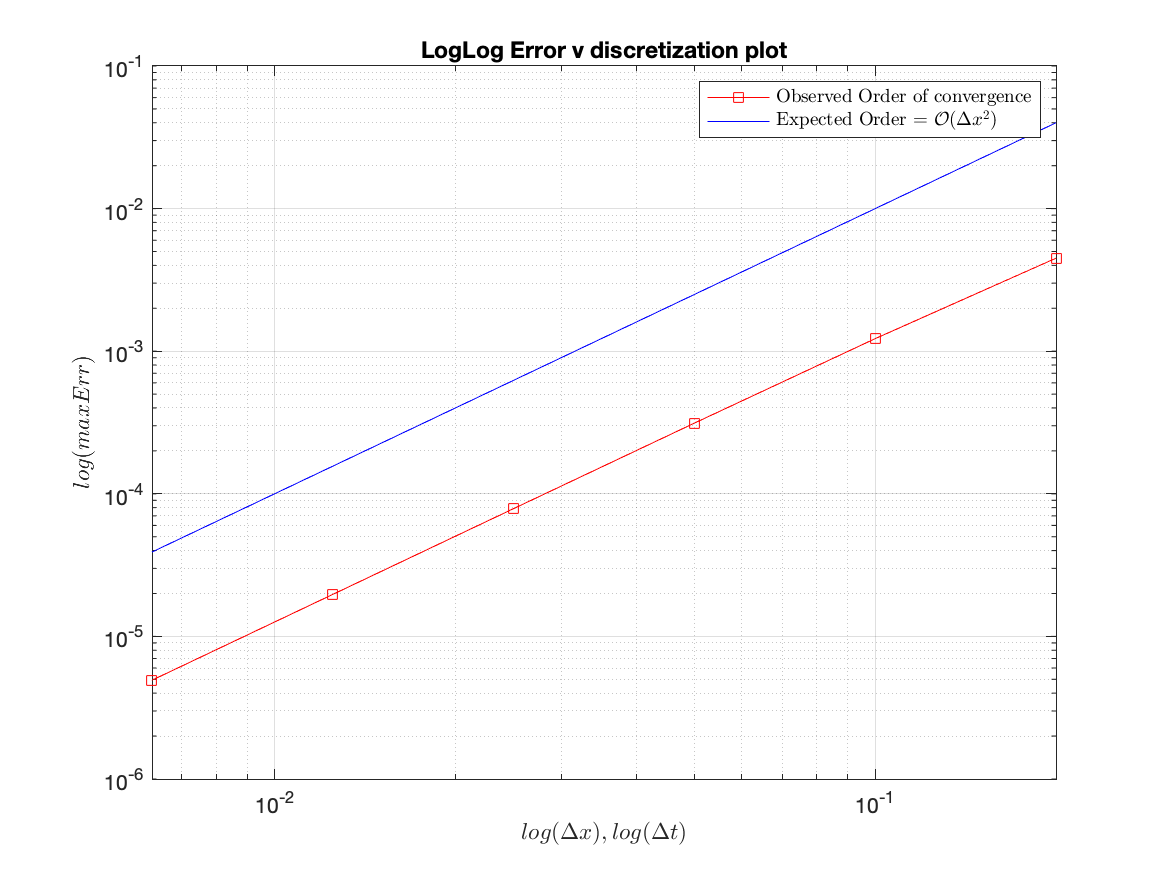
\includegraphics[width=4.2in]{ErrPlotQ1.png}
        \caption{Order of Convergence plot}
        \label{fig:convergence_q1}
    \end{figure}
  \end{enumerate}
  
  %%%%%
  %%%%%
  %%%%%
  \item (25 pts.) {\color{red}Consider a heat conduction problem in an annular section}
  \[
    u_{t} = \nu\left[\frac{1}{r}(ru_r)_r+\frac{1}{r^2}u_{\theta\theta}\right], \quad 1<r<2, \quad 0<\theta<\frac{\pi}{2}, \quad t>0
  \]
  {\color{red}with initial condition }$u(r,\theta,0)=u_0(r,\theta)${\color{red}, and boundary conditions}
  \begin{align*}
    u_r(1,\theta,t) = \alpha_1(\theta,t), \qquad & u_r(2,\theta,t) = \alpha_2(\theta,t) \\
    u(r,0,t) = \beta_1(r,t) \qquad & u(r,\frac{\pi}{2},t) = \beta_2(r,t).
  \end{align*}
  %%%
  \begin{enumerate}
    \item {\color{blue}Write a second-order accurate code to solve this problem using centered differencing and Crank-Nicolson time integration.} \\
    \begin{align*}
        -\frac{r_1}{2r_{j,k}}r_{j-\h,k}v^{n+1}_{j-1,k} +& \bra{1+\frac{r_1}{2r_{j,k}} \bra{r_{j+\h,k}+r_{j-\h,k}} + \frac{r_2}{r^2_{j,k}} }v^{n+1}_{j,k} - \frac{r_1}{2r_{j,k}}r_{j+\h,k}v^{n+1}_{j+1,k}  \\
        &-\frac{r_2}{2r^2_{j,k}}v^{n+1}_{j,k-1} - \frac{r_2}{2r^2_{j,k}}v^{n+1}_{j,k+1} = \frac{r_1}{2r_{j,k}}r_{j-\h,k}v^{n}_{j-1,k} +\\ &\bra{1-\frac{r_1}{2r_{j,k}}\bra{r_{j+\h,k}+r_{j-\h,k}}-\frac{r_2}{r^2_{j,k}}}v^n_{j,k}+ \\
        & \frac{r_1}{2r_{j,k}}r_{j+\h,k}v^n_{j+1,k} + \frac{r_2}{2r^2_{j,k}}v^n_{j,k-1} + \frac{r_2}{2r^2_{j,k}}v^n_{j,k+1} + \dt\hat{F} \\
        & j=0,1,2,\ldots \ldots,N_r-1,N_r \\
        & k=0,1,2,\ldots \ldots, N_\theta -1, N_\theta 
    \end{align*}
    Boundary conditions are given by,
    \begin{align*}
        \frac{v^{n+1}_{1,k}-v^{n+1}_{-1,k}}{2\Delta r} =& \ \alpha_1\bra{r=1,\theta,(n+1)\Delta t} & \frac{v^{n+1}_{j,-1}+v^{n+1}_{j,1}}{2} =& \ \beta_1\bra{r,\theta=0,(n+1)\Delta t} \\ \\
        \frac{v^{n+1}_{N_r+1,k}-v^{n+1}_{N_r-1,k}}{2\Delta r} =& \ \alpha_2\bra{r=2,\theta,(n+1)\Delta t} & \frac{v^{n+1}_{j,N_\theta-1}+v^{n+1}_{j,N_\theta +1}}{2} =& \ \beta_2\bra{r,\theta=\frac{\pi}{2},(n+1)\Delta t} \\
    \end{align*}
    The code written for this is shown in Listing~\ref{lst:mesh_gen}, Listing~\ref{lst:HE_mapping}, and Listing~\ref{lst:code_reconstruct}. 
    \lstinputlisting[caption={Mesh Generation code},label={lst:mesh_gen},language=Matlab]{genMesh.m}
    \lstinputlisting[caption={Heat Equation 2D under domain mapping},label={lst:HE_mapping},language=Matlab]{HeatEqn2DMapping.m}
    \lstinputlisting[caption={Reconstructing solution code},label={lst:code_reconstruct},language=Matlab]{reconstructSol.m}
    %
    \item {\color{blue}Verify the accuracy of your code using manufactured solutions.} \\
    \begin{align*}
        u\bra{r,\theta,t} =& \ \cos{\bra{\pi r}}\sin{2\theta}\sin{t}, \, r\in \bra{1,2}, \, \theta \in \bra{0,\frac{\pi}{2}}\\
        u_r\bra{r,\theta,t} =& \ -\pi\sin{\bra{\pi r}}\sin{2\theta}\sin{t} \\
        u_t\bra{r,\theta,t} =& \ \cos{\bra{\pi r}}\sin{2\theta}\cos{t} \\
        \frac{1}{r}\bra{ru_r}_r =& \ -\pi\sin{2\theta}\sin{t}\bra{\frac{\sin{\pi r}}{r} + \pi\cos{\pi r}} \\
        \frac{1}{r^2}\bra{u_{\theta\theta}} =& \ -\frac{4}{r^2}\cos{\bra{\pi r}}\sin{2\theta}\sin{t}
    \end{align*}
    \[
        f(r,\theta,t) = u_t - \nu\bra{\frac{1}{r}\bra{ru_r}_r + \frac{1}{r^2}u_{\theta\theta}}
    \]
    Boundary conditions are, 
    \begin{align*}
        u_r\bra{r=1} =& \ 0, & u\bra{\theta=0} =& \ 0 \\
        u_r\bra{r=2} =& \ 0, & u\bra{\theta=\frac{\pi}{2}} =& \ 0 
    \end{align*}
    The order of convergence is shown in Fig~\ref{fig:convergence_2D}. 
    \begin{figure}[htp]
        \centering
        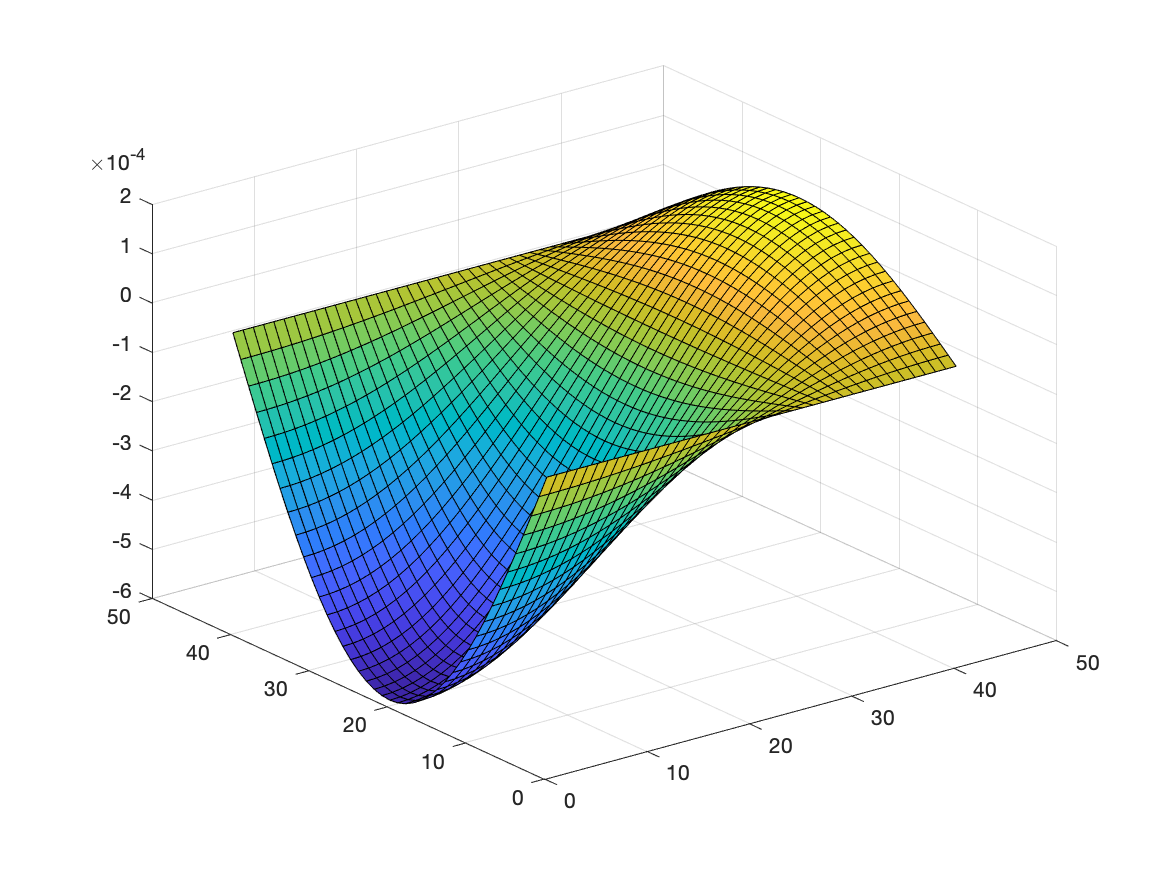
\includegraphics[width=5in]{ErrPlotQ2.png}
        \caption{Order of Convergence}
        \label{fig:convergence_2D}
    \end{figure}
    %
    \item {\color{blue}Now set} 
    \begin{align*}
      u_0(r,\theta) & = 0\\
      \alpha_1(\theta,t) & = 0\\
      \alpha_2(\theta,t) & = 0\\
      \beta_1(r,t) & = 0\\
      \beta_2(r,t) & = (r-1)^2(r-2)^2.
    \end{align*}
    {\color{blue}Using $\nu=1$ and 40 grid lines in both the radial and angular coordinate directions, compute numerical solutions to this problem at $t=0,.1,.5,1.5$. Create surface plots of the solution for each time. }\\
    The solutions are plotted in Fig~\ref{fig:HE2D_annulus} and Fig~\ref{fig:HE2D_annulus2}. 
    \begin{figure}[htp]
        \centering
        \begin{tabular}{c}
            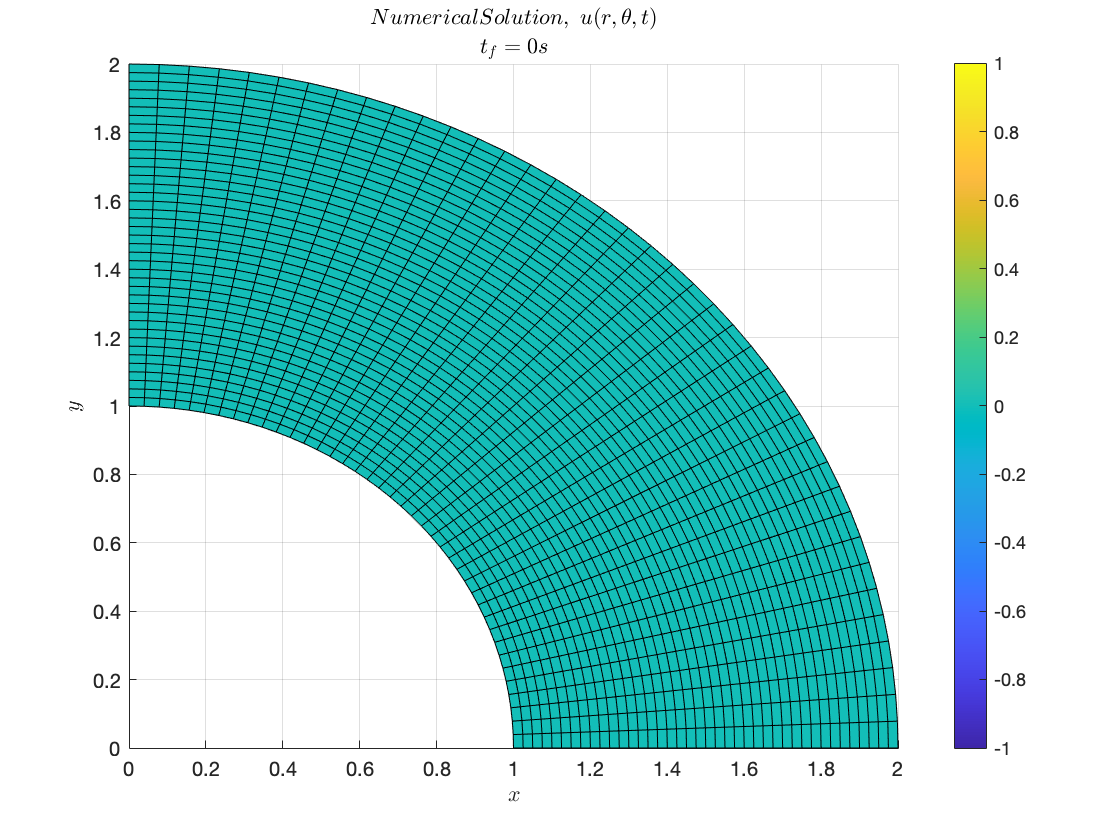
\includegraphics[width=5in]{Plot1.png} \\
            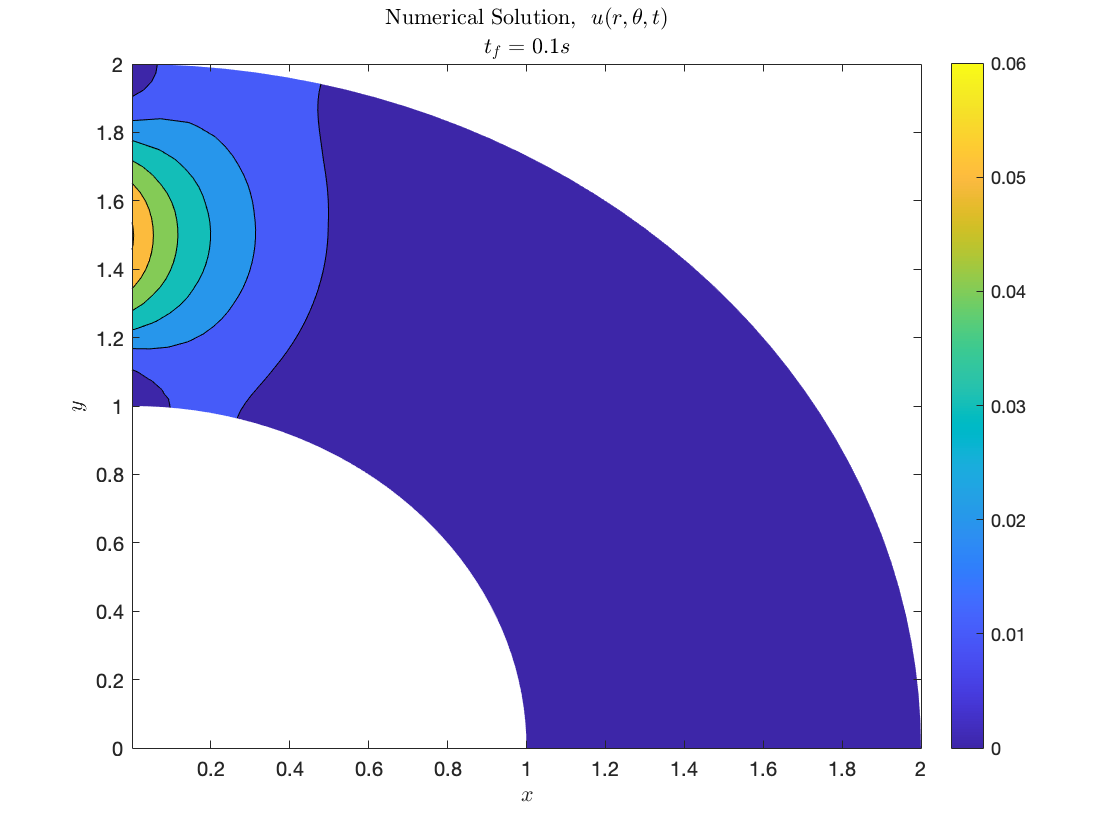
\includegraphics[width=5in]{Plot2.png} \\
        \end{tabular}
        \caption{Solution at different final times}
        \label{fig:HE2D_annulus}
    \end{figure}
    \begin{figure}[htp]
        \centering
        \begin{tabular}{c}
            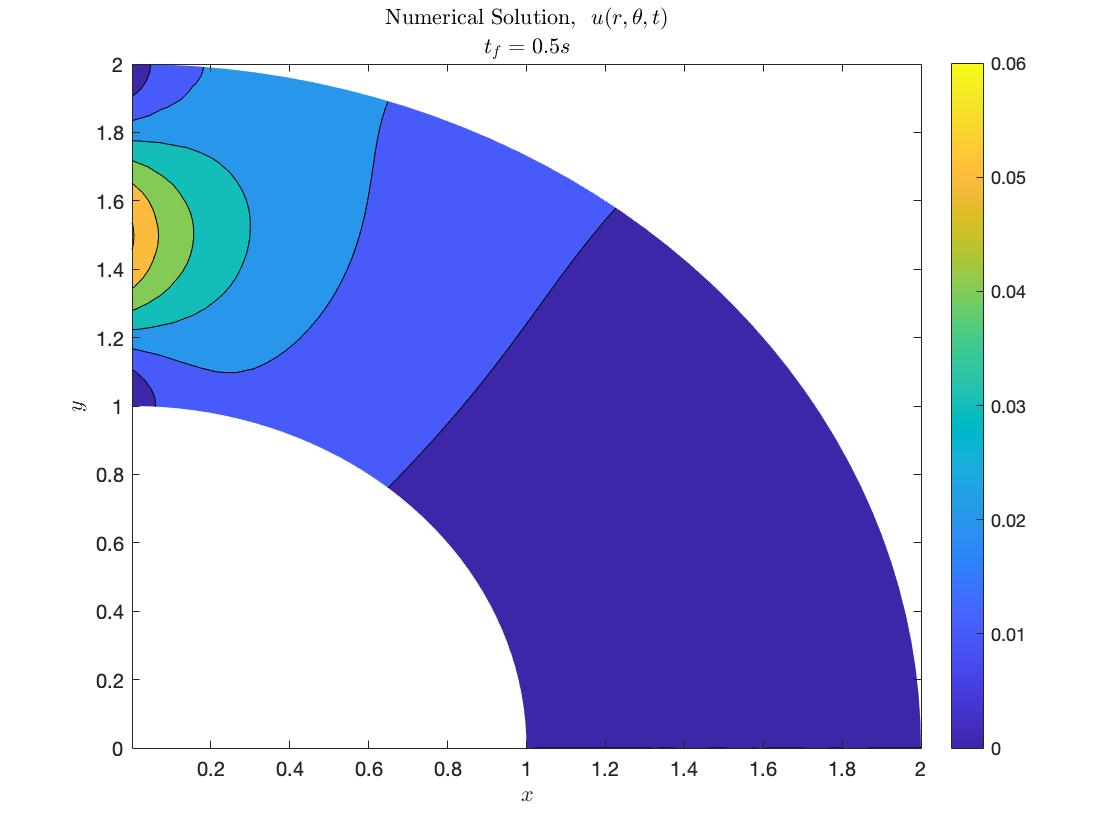
\includegraphics[width=5in]{Plot3.png} \\
            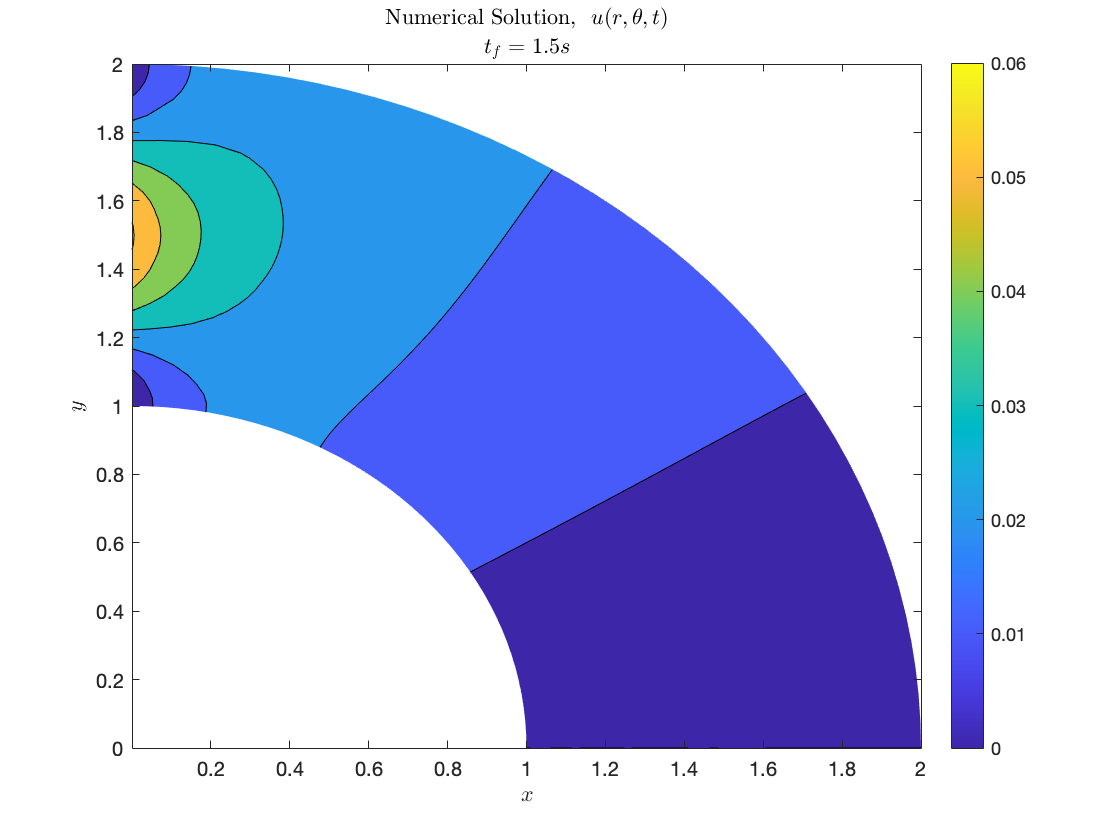
\includegraphics[width=5in]{Plot4.png} \\
        \end{tabular}
        \caption{Solution at different final times}
        \label{fig:HE2D_annulus2}
    \end{figure}
    %
    \item {\color{blue}Create a single line plot with four curves showing the solutions from part (c) along the inner radius ($r=1$), as a function of $\theta$ for all four times $t=0,.1,.5,1.5$.}\\
    The 1-D slice of the function is shown in Fig~\ref{fig:slice1D_1} and Fig~\ref{fig:slice1D_2}.
    \begin{figure}[htp]
        \centering
        \begin{tabular}{c}
            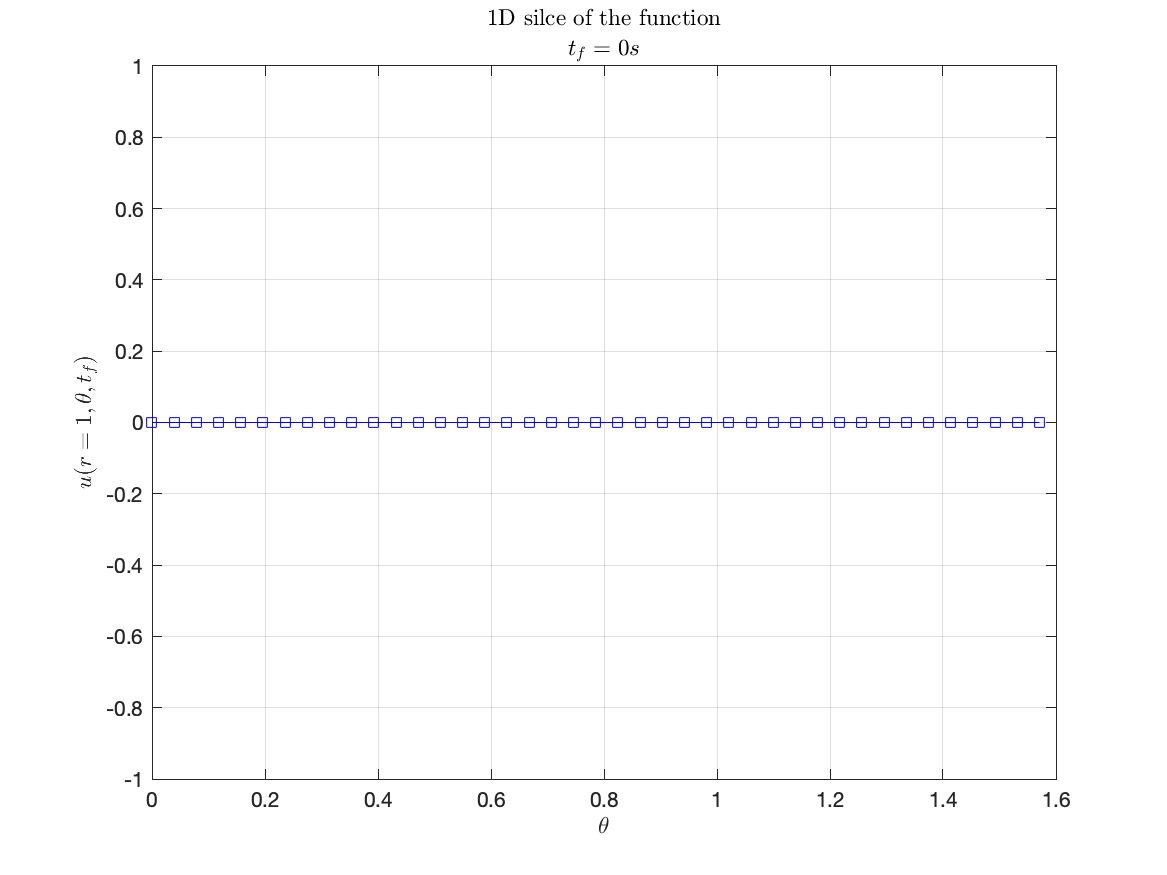
\includegraphics[width=5in]{Q2D_1.png}\\
            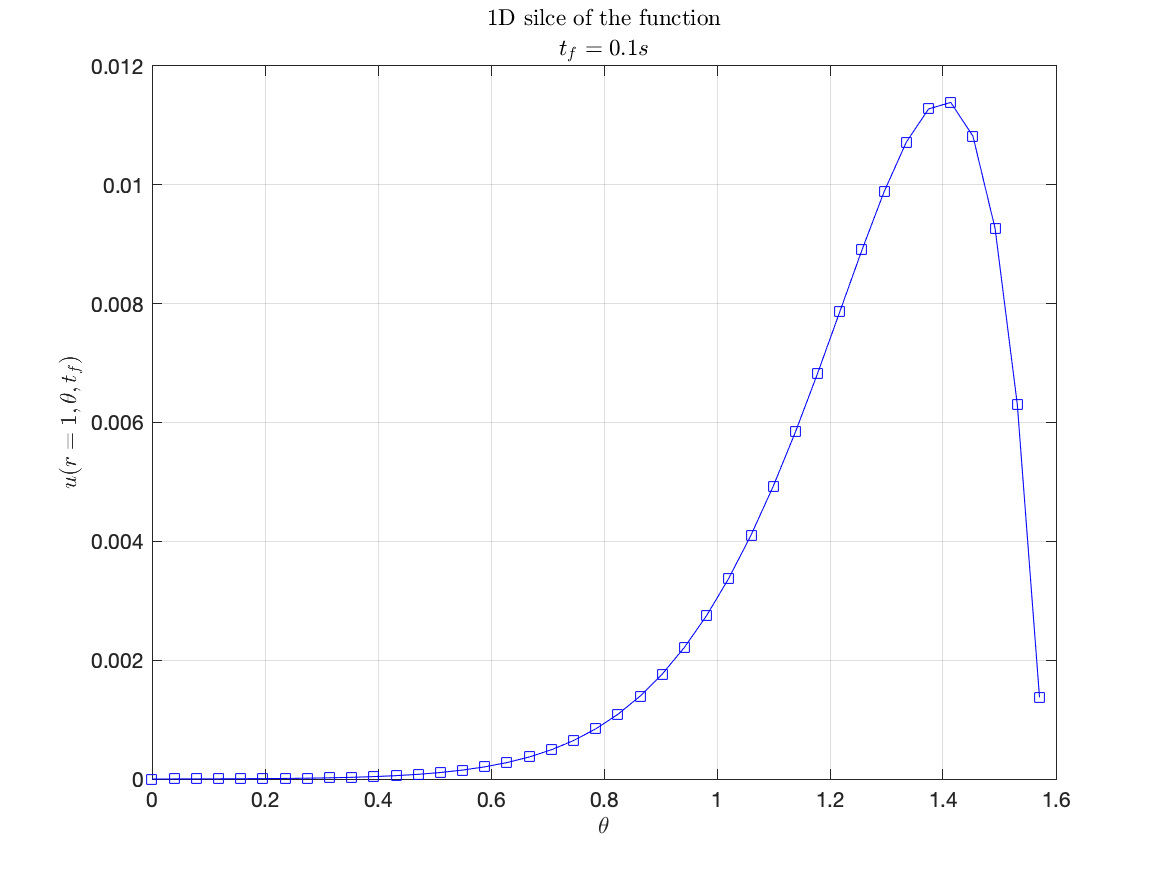
\includegraphics[width=5in]{Q2D_2.png}
        \end{tabular}
        \caption{1D slice of solution at final time - 1}
        \label{fig:slice1D_1}
    \end{figure}
    \begin{figure}[htp]
        \centering
        \begin{tabular}{c}
            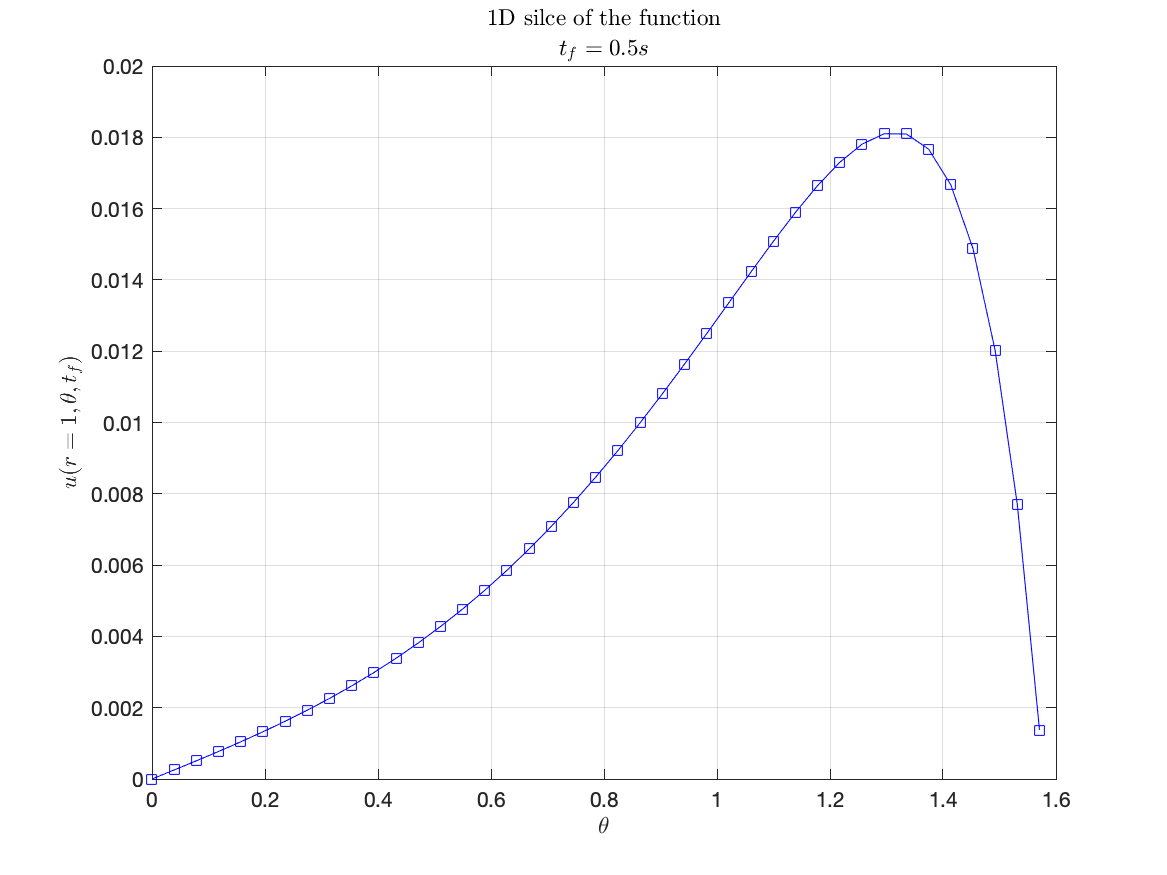
\includegraphics[width=5in]{Q2D_3.png}\\
            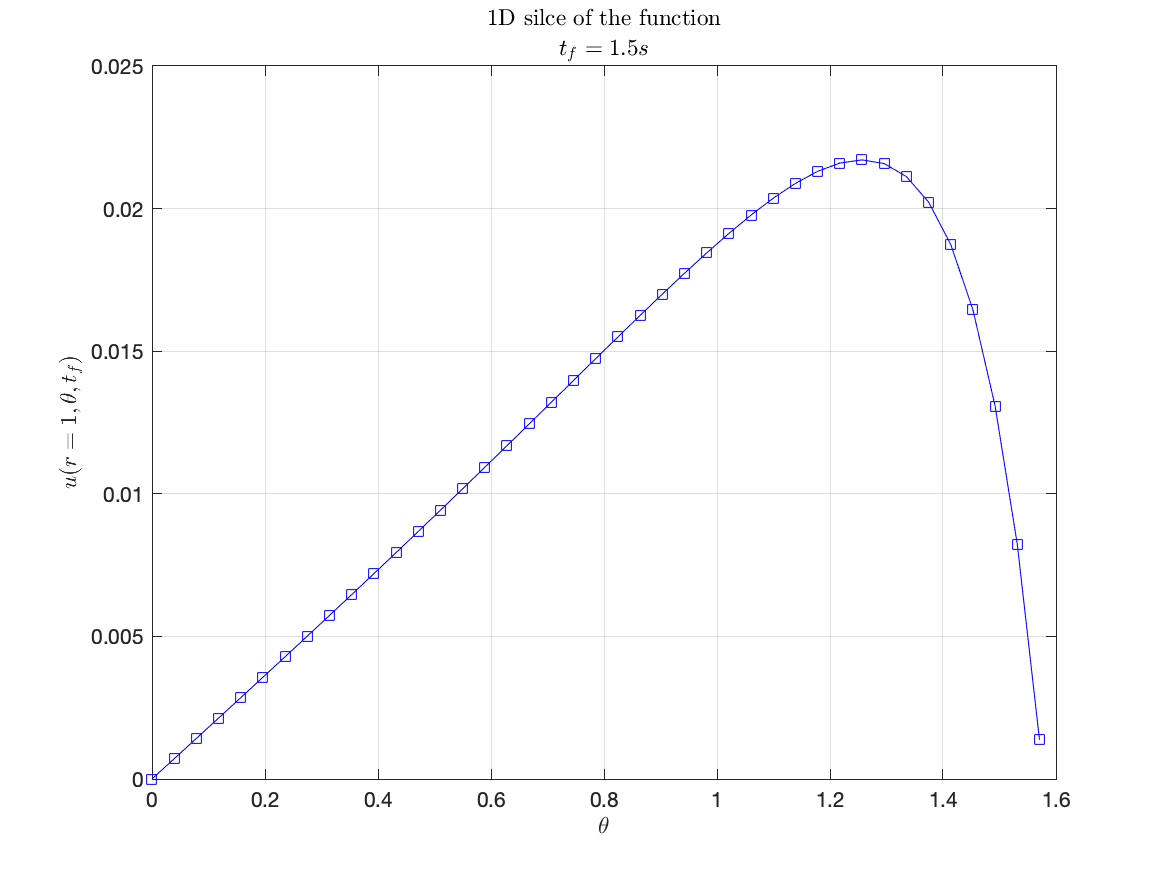
\includegraphics[width=5in]{Q2D_4.png}
        \end{tabular}
        \caption{1D slice of solution at final time - 2}
        \label{fig:slice1D_2}
    \end{figure}    
  \end{enumerate}
\end{enumerate}

\end{document}
